\documentclass[12pt]{article}

\usepackage[
	top    = 0.50in,
	left   = 1.25in,
	right  = 1.25in,
	bottom = 1.00in,
]{geometry}

\usepackage{amsmath, amssymb, latexsym, xcolor, graphicx, hyperref, tocloft}

\renewcommand \cftsecleader {\cftdotfill 3}
\renewcommand \contentsname {Table of Contents}
\def \combinedDocuments {}

\providecommand \darkMode 1
\ifnum \darkMode = 0 \else
	\pagecolor{black}
	\color[RGB]{170, 170, 170}
\fi

\begin{document}

\title{Physics 1 \& 2 for Engineers (PS 161) – Exam Formulas}
\author{Daniel E. Janusch}
\date{December 10, 2024}
\maketitle

\tableofcontents

\newpage \section{Exam 1 Formulas – Ch. 1-3} % this one might be missing formulas

\ifx \combinedDocuments \undefined
\documentclass[12pt]{article}

\usepackage[
	top    = 0.50in,
	left   = 1.25in,
	right  = 1.25in,
	bottom = 1.00in,
]{geometry}

\usepackage{amsmath, amssymb, latexsym, xcolor}

\providecommand \darkMode 1
\ifnum \darkMode = 0 \else
	\pagecolor{black}
	\color[RGB]{170, 170, 170}
\fi

\begin{document}

\newgeometry{
	top    = 0.00in,
	left   = 1.25in,
	right  = 1.25in,
	bottom = 1.00in,
}

\title{PS 161 Exam 1 Formulas}
\author{Daniel E. Janusch}
\date{December 9, 2024}
\maketitle
\fi

\begin{equation}
	v = v_0 + at
\end{equation}

\begin{equation}
	x = \dfrac{v_0 + v}t
\end{equation}

\begin{equation}
	x = v_0t + \dfrac a2 t^2
\end{equation}

\begin{equation}
	v^2 = v_0^2 + 2 a x
\end{equation}

\begin{equation}
	\text{vector stuff: dot, cross, angle, magnitude}
\end{equation}

\ifx \combinedDocuments \undefined
\end{document}
\fi

\newpage \section{Exam 2 Formulas – Ch. 4-5} % this one might be missing formulas

\ifx \combinedDocuments \undefined
\documentclass[12pt]{article}

\usepackage[
	top    = 0.50in,
	left   = 1.25in,
	right  = 1.25in,
	bottom = 1.00in,
]{geometry}

\usepackage{amsmath, amssymb, latexsym, xcolor}

\providecommand \darkMode 1
\ifnum \darkMode = 0 \else
	\pagecolor{black}
	\color[RGB]{170, 170, 170}
\fi

\begin{document}

\newgeometry{
	top    = 0.00in,
	left   = 1.25in,
	right  = 1.25in,
	bottom = 1.00in,
}

\title{PS 161 Exam 2 Formulas}
\author{Daniel E. Janusch}
\date{December 9, 2024}
\maketitle
\fi

\begin{equation}
	a_c = \dfrac{v^2} r
\end{equation}

\begin{equation}
	f_s = \mu_s N
\end{equation}

\begin{equation}
	f_k = \mu_k N
\end{equation}

\begin{equation}
	a_\parallel = g(\sin \theta - \mu_k \cos \theta) ~~ \text{box sliding down slope}
\end{equation}

\begin{equation}
	F = m a
\end{equation}

\ifx \combinedDocuments \undefined
\end{document}
\fi

\newpage \section{Exam 3 Formulas – Ch. 6-8} \providecommand \grav {\textrm{grav}}
\providecommand \cons {\textrm{cons}}
\providecommand \nc {\textrm{nc}}
\providecommand \el {\textrm{el}}
\providecommand \cm {\textrm{cm}}
\providecommand \av {\textrm{av}}

\providecommand \pvec {\hspace{-1px}\vec{\hspace{1px}p}}
\providecommand \vvec {\hspace{-1px}\vec{\hspace{1px}v}}

\providecommand \ds {\textrm ds}
\providecommand \dt {\textrm dt}
\providecommand \dU {\textrm dU}
\providecommand \dW {\textrm dW}
\providecommand \dx {\textrm dx}

\providecommand \DK {\Delta K}
\providecommand \DU {\Delta U}
\providecommand \DW {\Delta W}
\providecommand \Dy {\Delta y}
\providecommand \Dp {\Delta p}
\providecommand \Dt {\Delta t}

\ifx \combinedDocuments \undefined
\documentclass[12pt]{article}

\usepackage[
	top    = 0.50in,
	left   = 1.25in,
	right  = 1.25in,
	bottom = 1.00in,
]{geometry}

\usepackage{amsmath, amssymb, latexsym, xcolor}

\providecommand \darkMode 1
\ifnum \darkMode = 0 \else
	\pagecolor{black}
	\color[RGB]{170, 170, 170}
\fi

\begin{document}

\newgeometry{
	top    = 0.0in,
	left   = 1.25in,
	right  = 1.25in,
	bottom = 1.0in,
}

\title{PS 161 Exam 3 Formulas}
\author{Daniel E. Janusch}
\date{October 22, 2024}
\maketitle
\fi

\begin{equation}
	W = \int_{x_1}^{x_2} \! \vec F \cdot \vec \ds = W_\cons + W_\nc = \DK = \left. \left(\dfrac 12 mv^2~~\text{or}~~\dfrac{p^2}{2m}\right) \right|_{x_1}^{x_2}
\end{equation}

\begin{equation}
	W_F^\cons = -\DU_F
\end{equation}

\begin{equation}
	U_\grav = mgy ~~~~~~~~ U_\el = \dfrac 12 k x^2
\end{equation}

\begin{equation}
	J = \int_{t_1}^{t_2} \! F(t) \,\text dt = \Dp = mv \, \Big|_{t_1}^{t_2} = F_\av\Dt
\end{equation}

\begin{equation}
	F = -\vec \nabla U = \dot{m\vec v}
\end{equation}

\begin{equation}
	P_\av = \dfrac W \Dt ~~~~~~~~ P = \dot W = \vec F \cdot \vvec
\end{equation}

\begin{equation}
	\pvec = m\vvec
\end{equation}

\begin{equation}
	x_\cm = \dfrac{\sum mx}{\sum m} ~~~~~~~~ \vvec_\cm = \dfrac{\sum \pvec}{\sum m}
\end{equation}

\begin{equation}
	\DW = -\DU
\end{equation}

\begin{equation}
	v_{Af},v_{Bf} = \dfrac{p_{Ai} + 2 p_{Bi} - m_B v_{Ai}}{m_A + m_B}, \dfrac{p_{Bi} + 2 p_{Ai} - m_A v_{Bi}}{m_A + m_B}~~(\text{elastic})
\end{equation}

%% Terminal velocity?

\ifx \combinedDocuments \undefined
\end{document}
\fi
\newpage \section{Exam 4 Formulas – Ch. 9-11} 
\providecommand \hpx [1] {\hspace{#1px}}
\providecommand \vpx [1] {\vspace{ #1px}}
\providecommand \nhpx [1] {\hspace{-#1px}}
\providecommand \nvpx [1] {\vspace{-#1px}}

\providecommand \grav {\textrm{grav}}
\providecommand \rad {\textrm{rad}}
\providecommand \rot {\textrm{rot}}
\providecommand \lin {\textrm{lin}}
\providecommand \cm {\textrm{cm}}
\providecommand \cg {\textrm{cg}}
\providecommand \av {\textrm{av}}

\providecommand \pgrp [1] {\left( #1 \right)}

\providecommand \Fvec {\vec F}
\providecommand \pvec {\nhpx 1 \vec {\hpx 1 p}}
\providecommand \rvec {\nhpx 1 \vec {\hpx 1 r}}

\providecommand \dm {\mathrm dm}
\providecommand \dr {\mathrm dr}
\providecommand \DK {\Delta K}

\ifx \combinedDocuments \undefined
\documentclass[12pt]{article}

\usepackage[
	top    = 0.50in,
	left   = 1.25in,
	right  = 1.25in,
	bottom = 1.00in,
]{geometry}

\usepackage{amsmath, amssymb, latexsym, xcolor, graphicx}

\providecommand \darkMode 1
\ifnum \darkMode = 0 \else
	\pagecolor{black}
	\color[RGB]{170, 170, 170}
\fi

\begin{document}

\newgeometry{
	top    = 0.00in,
	left   = 1.25in,
	right  = 1.25in,
	bottom = 1.00in,
}

\title{PS 161 Exam 4 Formulas}
\author{Daniel E. Janusch}
\date{November 12, 2024}
\maketitle
\fi

\begin{equation}
	s = r \theta \hpx{20} v = r \omega \hpx{20} a = r \alpha
\end{equation}

\begin{equation}
	\omega = \omega_0 + \alpha t
\end{equation}

\begin{equation}
	\theta = \omega_\av t = \omega_0 t + \dfrac \alpha 2 t^2
\end{equation}

\begin{equation}
	\omega^2 = \omega_0^2 + 2 \alpha \theta
\end{equation}

\begin{equation}
	a_\rad = \dfrac{v^2}r = r \omega^2
\end{equation}

\begin{equation}
	I = \sum_{i=1}^N m_i r_i^2 = \int \! r^2 \hpx 1 \dm = \int \! r^2 \lambda(r) \dr
\end{equation}

\begin{equation}
	I = I_\cm + m d^2 \Longrightarrow I_2 = I_1 + m \! \pgrp{d_2^2 - d_1^2}
\end{equation}

\begin{equation}
	K_\rot = \dfrac 1 2 I \omega^2
\end{equation}

\begin{equation}
	W = \DK_\lin + \DK_\rot
\end{equation}

\begin{equation}
	U_\grav = m g y_\cm
\end{equation}

\begin{equation}
	\tau = \rvec \times \Fvec = F \ell = F_\perp r = r F \sin \theta = I \alpha = \dot L
\end{equation}

\begin{equation}
	x_\cg = x_\cm ~~~ (\textrm{usually})
\end{equation}

\begin{equation}
	\textrm{statics} \Longrightarrow \sum F = \sum \tau = 0
\end{equation}

\begin{equation}
	\textrm{rolling without slipping} \Longrightarrow v_\cm = r \omega ~~ \land ~~ a_\cm = r \alpha
\end{equation}

\begin{equation}
	P = \tau \omega
\end{equation}

\pagebreak
\restoregeometry

\begin{figure}[ht]
	\centering
	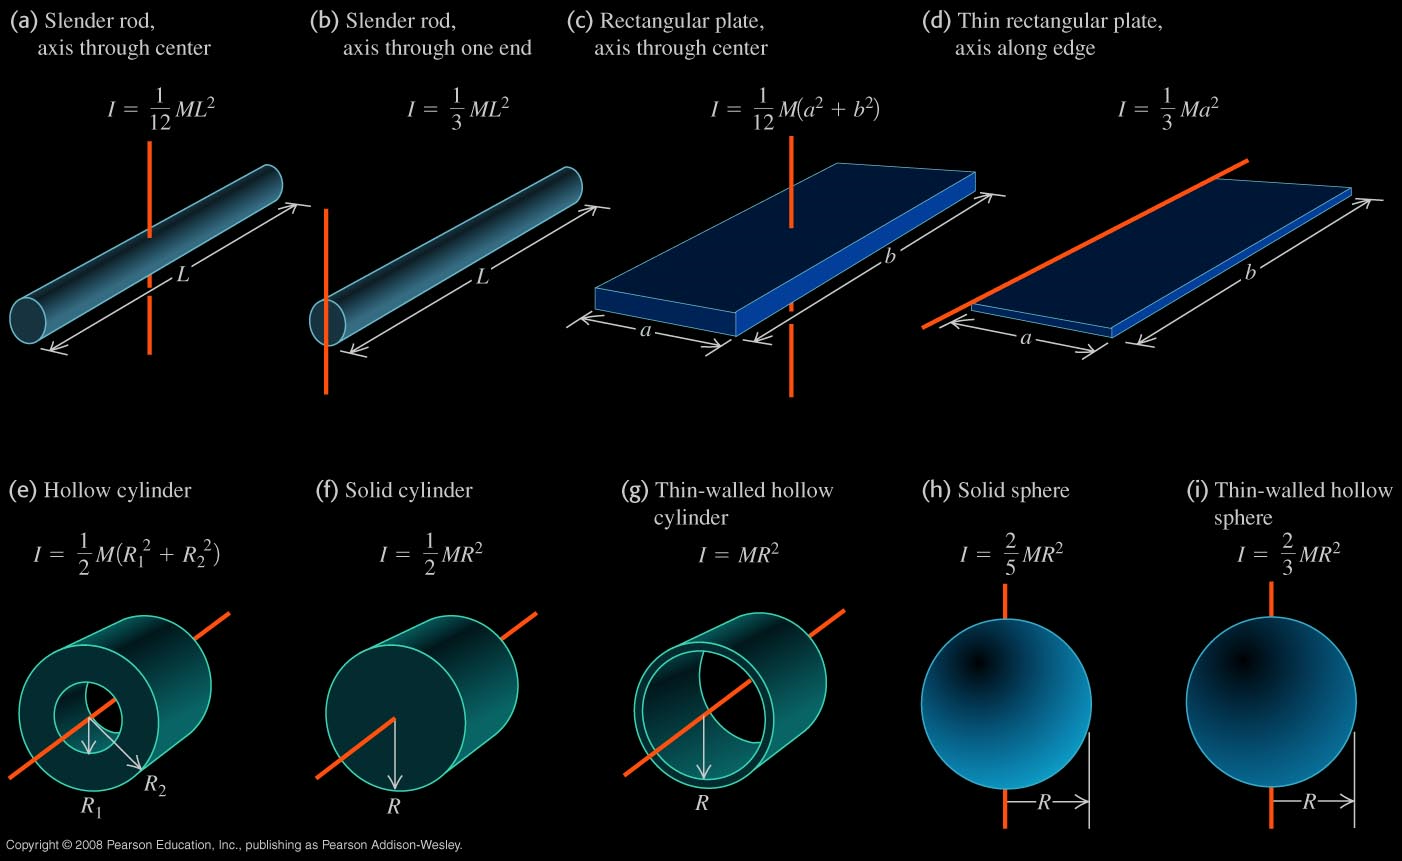
\includegraphics[width=\textwidth]{./rotational-inertia-table.png}
\end{figure}

\nvpx{20} \begin{equation}
	L = \rvec \times \pvec = mvr \sin \theta = mv\ell = I \omega
\end{equation}

\begin{equation}
	\hpx{36} L_0 = L_1 ~~~~ (\textrm{assuming no external torque})
\end{equation}

% \begin{equation}
% 	\Omega = \dot \phi = \dfrac \tau L = \dfrac{w r} {I \omega} ~~~~~ (\textrm{gyroscope})
% \end{equation}

% \begin{equation}
% 	\tau = \rvec_\cm \times \wvec
% \end{equation}

\ifx \combinedDocuments \undefined
\end{document}
\fi
\newpage \section{Final Exam Formulas – Ch. 12-14} \documentclass[12pt]{article}

\usepackage{amsmath, amssymb, latexsym, xcolor, graphics, hyperref, tocloft}

\usepackage[
	top    = 0.75in,
	left   = 1in,
	right  = 1in,
	bottom = 1in,
]{geometry}

\definecolor{lightgray}{RGB}{170, 170, 170}

\color{lightgray}
\pagecolor{black}

\newcommand \dstyle \displaystyle
\newcommand \hpx [1]{\hspace{#1px}}
\newcommand \vpx [1]{\vspace{#1px}}
\newcommand \nhpx [1]{\hspace{-#1px}}
\newcommand \nvpx [1]{\vspace{-#1px}}

\renewcommand \cftsecleader {\cftdotfill 3}
\renewcommand \contentsname {Table of Contents}
\renewcommand \implies {\ensuremath{\hpx 4 \raisebox{-0.14px}{\scalebox{1.051} =} \nhpx{5.2} \Rightarrow \hpx 3}}
\renewcommand \d {\mathrm d}

\newcommand \E [1] {\textsc{e}\!#1\!}
\newcommand \eps \varepsilon
\newcommand \emf {\mathcal E}
\newcommand \eq {\mathrm{eq}}

\newcommand \dt {\d t}
\newcommand \dx {\d x}
\newcommand \dq {\d q}
\newcommand \dI {\d I}
\newcommand \dV {\d V}
\newcommand \dQ {\d Q}
\newcommand \dA {\d A}

\newcommand \A {\mathrm A} % amp
\newcommand \C {\mathrm C} % coulomb
\newcommand \F {\mathrm F} % farad
\newcommand \G {\mathrm G} % gauss
\renewcommand\H{\mathrm H} % henry
\newcommand \J {\mathrm J} % joule
\newcommand \N {\mathrm N} % newton
\newcommand \T {\mathrm T} % teslas
\newcommand \V {\mathrm V} % volt
\newcommand \W {\mathrm W} % watt

\newcommand \s {\mathrm s} % second
\newcommand \m {\mathrm m} % meter

\newcommand \kg {\mathrm{kg}} % kilogram
\newcommand \eV {\mathrm{eV}} % electron volt
\newcommand \Wb {\mathrm{Wb}} % weber
\newcommand \rad{\mathrm{rad}}% radian

\begin{document}

\newgeometry{
	top    = 0in,
	left   = 1in,
	right  = 1in,
	bottom = 1in,
}

\title{PS 250 Final Exam Formula Sheet Plan}
\author{Daniel E. Janusch}
\maketitle
\vpx{-30}

\tableofcontents

\vfill
$\hfill \text{\scriptsize NOTE: The LaTeX source has more context in comments for some formulas}$

\newpage
\restoregeometry

\section{Constants} \setcounter {equation} 0

\begin{equation}
	\eps_0 = 8.8541878188\E-12 ~~~~ \left[\dfrac \F \m \right]
\end{equation}

\begin{equation}
	k = \dfrac 1 {4 \pi \eps_0} = 8.987551787\E+9 ~~~~ \left[\dfrac \m \F \right]
\end{equation}

\begin{equation}
	e = 1.602176634\E-19 ~~~~ [\C]
\end{equation}

\begin{equation}
	m_e = 9.10938356\E-31 ~~~~ [\kg]
\end{equation}

\begin{equation}
	m_p = 1.672621898\E-27 ~~~~ [\kg]
\end{equation}

\begin{equation}
	m_n = 1.674927471\E-27 ~~~~ [\kg]
\end{equation}

\begin{equation}
	\mu_0 = 4\pi \times 10^{-7} ~~~~ \left[\dfrac{\T \; \m} \A \right]
\end{equation}

\begin{equation}
	c = 299\;792\;458 ~~~~ \left[\dfrac \m \s\right]
\end{equation}

\begin{equation}
	h = 2 \pi \hbar = 6.62607015\E-34 ~~~ [\J \; \s]
\end{equation}

\begin{equation}
	\mu_B = 9.27401022241938\E-24 ~~~~ \left[\dfrac \J \T \right]
\end{equation}

\newpage

\section{Units} \setcounter {equation} 0

$\hfill \textrm{exponents (negative): } c, m, \mu, n, p = 2, 3, 6, 9, 12 \hfill$

\begin{equation}
	\C = \A \; \s
\end{equation}

\begin{equation}
	\V = \A \; \Omega = \dfrac \W \A = \dfrac \J \C = \dfrac{\kg \; \m^2}{\C \; \s^2}
\end{equation}

\begin{equation}
	\N = \dfrac{\kg \; \m}{\s^2}
\end{equation}

\begin{equation}
	\W = \dfrac \J \s
\end{equation}

\begin{equation}
	\J = \N \; \m = \V \; \C = \dfrac{\kg \; \m^2}{\s^2}
\end{equation}

\begin{equation}
	\eV = |e| \, \V
\end{equation}

\begin{equation}
	\F = \dfrac \C \V = \dfrac{\s^2 \; \C^2}{\kg \; \m^2} = \dfrac {\C^2} \J = \dfrac \s \Omega
\end{equation}

\begin{equation}
	\T = \dfrac \N {\A \; \m} = \dfrac \kg {\C \; \s} = 10^4 \, \G
\end{equation}

\begin{equation}
	\Wb = \V \; \s = \T \; \m^2 = \Omega \; \C = \dfrac \J \A
\end{equation}

\begin{equation}
	\H = \Omega \; \s = \dfrac \Wb \A = \dfrac {\s^2} \F = \dfrac {\Omega \; \s} \rad
\end{equation}

\begin{equation}
	\dfrac {\T \; \m} \A = \dfrac \H \m = \dfrac \N {\A^2}
\end{equation}

\begin{equation}
	\dfrac \V \m = \dfrac \N \C
\end{equation}

\newpage

\section{Realistic Value Ranges}
% these are all approximate, so if you get like 10 or 100 times larger, it should be fine in most cases.
% except for \eps / \eps_0, where 10 is basically the max you should see (probably, idk).

$\hfill \begin{array}{c|c}
	\text{range}					& \text{unit}	\\ \hline
	I \sim [10^{-4}, 10]			& \A			\\ % current
	v_e \sim 10^6					& \m / \s		\\ % electron absolute velocity
	v_d \sim 10^{-4}				& \m / \s		\\ % electron drift velocity
	n \sim 10^{28}					& \m^{-3}		\\ % free electron count thing
	C \sim [10^{-12}, 10^{-3}]		& \F			\\ % self capacitance
	R \sim [1, 10^3]				& \Omega		\\ % resistance
	V \sim [1, 200]					& \V			\\ % voltage
	P \sim [10^{-3}, 10^4]			& \W			\\ % power
	\rho \sim [10^{-9}, 10^{-6}]	& \Omega \; \m	\\ % resistivity
	E_c \sim [10^3, 10^7]			& \V / \m		\\ % capacitor electric field
	E_w \sim [10^{-3}, 10]			& \V / \m		\\ % wire electric field
	R_w \sim [10^{-3}, 10^{-2}]		& \Omega		\\ % wire resistance.
	B \sim [10^{-6}, 10]			& \T			\\ % magnetic field

	F_E \sim [10^{-12}, 10^2]		& \N			\\ % generic electric force
	F_B \sim [10^{-12}, 10]			& \N			\\ % generic magnetic force

	\Phi_E \sim [10^{-12}, 10]		& \V \; \m		\\ % electric flux
	\Phi_B \sim [10^{-8}, 1]		& \Wb			\\ % magnetic flux

	\eps/\eps_0 \sim [1, 10]		& \text{none}	\\ % dielectric constant
	\mu/\mu_0 \sim [1, 10^3]		& \text{none}	\\ % magnetic dielectric constant thing

	N \sim [1, 10^3]				& \text{none}	\\ % number of coils
	L \sim [10^{-9}, 10^2]			& \H			\\ % self inductance
	M \sim [10^{-9}, 10^{-3}]		& \H			\\ % mutual inductance
\end{array} \hfill$

\vpx{20}

\section{Resistivity Table}

$\hfill \text{\begin{tabular}{c|c}
	material	& resistivity	\\ \hline
	silver		& $1.6\E-8$		\\
	copper		& $1.7\E-8$		\\
	gold		& $2.2\E-8$		\\
	aluminum	& $2.6\E-8$		\\
	iron 		& $9.7\E-8$		\\
\end{tabular}} \hfill$

\newpage

\section{Electric Field ($E$, $F_E$, $\Phi_E$), Energy, Work, Voltage} % Exam 1 Formulas

\subsection{General Formulas} \setcounter {equation} 0

\begin{equation}
	F_E = k \dfrac{\left|q_1 q_2\right|}{r^2}
\end{equation}

\begin{equation}
	E = \dfrac F {q_t} = k \dfrac{|Q|}{r^2} = -\nabla V = -\dfrac \dV \dx
\end{equation}

\begin{equation}
	W = -\Delta U = q_t \Delta V = \int {\bf F} \cdot {\rm d}{\bf r}
\end{equation}

\begin{equation}
	W = q_t E d~~~(\textrm{uniform field. $d$ is the displacement})
\end{equation}

\begin{equation}
	U = k \dfrac{q_1 q_2} r
\end{equation}

\begin{equation}
	U_{\rm sys} = k \sum_{i < j} \dfrac{q_i q_j}{r_{i,j}}
\end{equation}

\begin{equation}
	\Phi_E = \oint {\bf E} \cdot {\rm d}{\bf A} = \dfrac{Q_{\rm encl}}{\eps_0}
\end{equation}

\begin{equation}
	V = \sum k \dfrac{Q_i}{r_i} = \dfrac U {q_t} = \int \dfrac \dq r
\end{equation}

\begin{equation}
	E_{\rm tot} = \sum_i E_i
\end{equation}

\subsection{Extended Objects}

\subsubsection{Voltage} \setcounter {equation} 0

\begin{equation}
	% also the same as for a line of charge.
	\text{Conducting Cylinder radius $R$: } V = 2 k \lambda \ln \dfrac R d \text{ if $d > R$ else 0}
\end{equation}

\begin{equation}
	\text{Ring: } V = \dfrac{k Q}{\sqrt{d^2 + R^2}}
\end{equation}

\newpage

\subsubsection{Electric Field} \setcounter {equation} 0

$\hfill\text{$E = 0$ inside a conducting region.}\hfill$

\begin{equation}
	% line goes from x=-a to x=b, where y=r is the distance away from x=0.
	\text{Line: } E = \dfrac{k \lambda} r \left[\dfrac a{\sqrt{a^2 + r^2}} + \dfrac b{\sqrt{b^2 + r^2}}\right] \approx \dfrac{2 k \lambda} r
\end{equation}

\begin{equation}
	% radius R disk
	\text{Disk/Plate: } E = \dfrac \sigma{2 \eps_0} \left[1 - \dfrac d{\sqrt{d^2 + R^2}}\right] \approx \dfrac \sigma{2 \eps_0} = 2 \pi k \sigma
\end{equation}

\begin{equation}
	% radius R ring. distance d perpendicular to it from the center.
	\text{Ring: } E = \dfrac{k Q d}{\left(d^2 + R^2\right)^{3/2}}, Q = 2 \pi R \lambda
\end{equation}

\begin{equation}
	\text{radius $R$ Sphere: } E = k \dfrac Q {r^2}, \text{ if } r \ge R
\end{equation}

\begin{equation}
	% r < R.
	% for a conducting sphere, E = 0 inside.
	\text{inside radius $R$ insulating Sphere: } E = \dfrac {k Q r} {R^3}
\end{equation}

\begin{equation}
	\text{radius $R$ cylinder: } E = \dfrac {2 k \lambda} r, \text{ if } r \ge R
\end{equation}

\begin{equation}
	% r < R
	% any non-conducting cylinder.
	% for a conducting cylinder, E = 0 inside.
	\text{inside radius $R$ insulating cylinder: } E = \dfrac {2 k \lambda r} {R^2}
\end{equation}

\begin{equation}
	\text{equal, opposite plates: } E = \dfrac \sigma {\eps_0} \text{ inside, else } 0
\end{equation}

\newpage

\section{Magnetism}

\subsection{General Formulas} \setcounter {equation} 0

\begin{equation}
	\vec F = F_E + F_B = q (\vec E + \vec v \times \vec B) \implies |\vec F| = q (E + v B \sin \theta)
\end{equation}

\noindent \text{this next one assumes magnetic field is orthogonal to motion:}

\begin{equation}
	F_B = (\text{\# of charges}) \left(\dfrac{\rm force}{\rm charge}\right)
		= (n A \ell)(q v B)
		= (n q v_d A) (\ell B)
		= I \ell B
\end{equation}

\begin{equation}
	\vec F_B = q \vec v \times \vec B = I \vec \ell \times \vec B
\end{equation}

\begin{equation}
	\vec \mu = N I \vec A ~~ (\text{magnetic moment})
\end{equation}

\begin{equation}
	\vec \tau = N I \vec A \times \vec B = \vec \mu \times \vec B ~~ (\text{torque})
\end{equation}

\begin{equation}
	U = \int \tau \d\theta = -\vec \mu \cdot \vec B ~~ (\text{magnetic potential energy})
\end{equation}

\begin{equation}
	\text{point charge: } B = 10^{-7} \dfrac{q \vec v \times \hat r}{r^2}
\end{equation}

\begin{equation}
	% R is the radius of the arc the particle goes in.
	\text{point charge: } m v = |q| B R
\end{equation}

\begin{equation}
	\oint \vec B \cdot \d\ell = \mu_0 I_{\rm encl}
\end{equation}

\begin{equation}
	\emf = - N \dfrac{\d\Phi_B} \dt = - N \dfrac{\d(A B \cos \theta)} \dt = B \ell v \sin \theta = I R
\end{equation}

\begin{equation}
	% r hat is from the source to the test location
	\vec B = 10^{-7} \int \dfrac{I \d\ell \times \hat r}{r^2}
\end{equation}

\begin{equation}
	%  B_\perp
	\Phi_B = \int B \cos \theta \dA = \int \vec B \cdot \d\vec A = A B \cos \theta
\end{equation}

\begin{equation}
	\oint \vec B \cdot \d\vec A = 0
\end{equation}

\begin{equation}
	\text{velocity selector: } F_E = F_B \implies v = \dfrac E B
\end{equation}

\begin{equation}
	% magnetic force between two wires
	% this is really F_i / L_i, but usually L_1 = L_2.
	% F_1 / L_1 = F_2 / L_2.
	% same current direction => attract
	% opposite current direction => repel
	\dfrac F L = \dfrac {\mu_0 I_1 I_2} {2 \pi r}
\end{equation}

\newpage

\subsection{Ampere's Law Applications} \setcounter {equation} 0

$\hfill \text{magnetic field outside a solenoid is zero} \hfill$

\begin{equation}
	\text{cylindrical solenoid: } B = \mu_0 n I = \mu_0 \dfrac N \ell I
\end{equation}

\begin{equation}
	\text{toroidal solenoid: } B = \dfrac{\mu_0}{2 \pi} N \dfrac I r, r_{\rm min} < r < r_{\rm max}
\end{equation}

\begin{equation}
	\text{distance $r$ away from a radius-$R$ wire center: } B = \dfrac{\mu_0}{2 \pi} \begin{cases}
		\vpx 5
		\dfrac {I r} {R^2}, r < R \\
		\dfrac I r, r \ge R
	\end{cases}
\end{equation}

\begin{equation}
	% assumes I is either into or out of the page.
	\text{torus of current at $a < r < b$: } B = \dfrac {\mu_0} {2 \pi} \dfrac I r \begin{cases}
		0, r < a \\
		\dfrac {r^2 - a^2} {b^2 - a^2}, a < r < b \\
		1, b < r \\
	\end{cases}
\end{equation}

\newpage

\section{General DC Circuit Formulas} \setcounter {equation} 0

\begin{equation}
	V = \dfrac Q C, ~ I = C \dfrac \dV \dt
\end{equation}

\begin{equation}
	R = \dfrac V I = \dfrac {\rho \ell} A
\end{equation}

\begin{equation}
	L = \dfrac {N \Phi_B} I = \dfrac {A B N} I
\end{equation}

\begin{equation}
	M = \dfrac {N_2 \Phi_{B2}} {I_1} = \dfrac {N_1 \Phi_{B1}} {I_2}
\end{equation}

\begin{equation}
	\emf = - L \dfrac \dI \dt, ~ \emf_1 = - M \dfrac {\dI_2} \dt, ~ \emf_2 = - M \dfrac {\dI_1} \dt
\end{equation}

\begin{equation}
	\hfill \begin{array}{c|cc}
		\text{equivalences}	& \text{Series}		& \text{Parallel}	\\ \hline
		\text{Capacitor}	& [\sum 1/C_i]^{-1}	& \sum C_i			\\
		\text{Resistor}		& \sum R_i			& [\sum 1/R_i]^{-1} \\
		\text{Inductor}		& \sum L_i			& [\sum 1/L_i]^{-1} \\
	\end{array} \hfill
\end{equation}

\begin{equation}
	U_C = \dfrac 1 2 \dfrac{Q^2} C = \dfrac 12 C V^2 = \dfrac 1 2 Q V, ~ U_L = \dfrac 1 2 L I^2
\end{equation}

\begin{equation}
	% energy density.
	u_C = \dfrac {\eps_0} 2 \dfrac {V^2}{d^2} = \dfrac {\eps_0} 2 E^2, ~
	u_L = \dfrac {B^2} {2 \mu_0}
\end{equation}

\begin{equation}
	\text{dielectric: } C = K C_0,~K = \dfrac{C}{C_0} = \dfrac{\eps}{\eps_0}
\end{equation}

\begin{equation}
	I = \dfrac \dQ \dt = |q| n A v_d
\end{equation}

\begin{equation}
	J = \dfrac I A = \dfrac E \rho ~~ \text{(current density)}
\end{equation}

\begin{equation}
	P_R = V I = \dfrac{V^2} R = I^2 R, ~ P_L = I L \dfrac \dI \dt
\end{equation}

\begin{equation}
	I = L \dfrac \dI \dt
\end{equation}

% equal and opposite parallel plates (capacitor)
\begin{equation}
	\text{parallel plate: }
		C = \dfrac Q V = \dfrac{\eps A} d,
		E = \dfrac V d = \dfrac Q {C d} = \dfrac Q {\eps A},
		d = \dfrac{\eps A} C = \dfrac{\eps A V} Q
\end{equation}

\begin{equation}
	\text{Junction/Current rule: } \sum I_{\rm in} = \sum I_{\rm out}
\end{equation}

\begin{equation}
	\text{Loop/Voltage rule: } \sum V = 0 ~~ \text{(around a closed loop)}
\end{equation}

$\hfill \text{charge is preserved in series, but split in sequence} \hfill$

\begin{equation}
	\text{series: } Q_\eq = C_\eq V_\eq, ~ V_i = \dfrac {C_\eq} {C_i} V_\eq
\end{equation}

\begin{equation}
	\text{parallel: } Q_i = C_i V_\eq = \dfrac {C_i} {C_\eq} Q_\eq, ~ V_i = V_\eq
\end{equation}

\begin{equation}
	\text{parallel, all equal: } Q_i = \dfrac {Q_\eq} n
\end{equation}

\newpage

\section{Inductors and Inductance Scenarios}

\subsection{Cylindrical Solenoid} \setcounter {equation} 0

\begin{equation}
	B = \mu_0 n I = \mu_0 \dfrac N \ell I
\end{equation}

\begin{equation}
	L = \dfrac {\mu_0 N^2 A} \ell
\end{equation}

\begin{equation}
	u_L = \dfrac {\mu_0 N^2 I^2} {2 \ell^2}
\end{equation}

\subsection{Toroidal Solenoid} \setcounter {equation} 0

\begin{equation}
	B = \dfrac{\mu_0}{2 \pi} N \dfrac I r, r_{\rm min} < r < r_{\rm max}
\end{equation}

\begin{equation}
	L = \dfrac{\mu_0 N^2 A}{2 \pi r_{\rm avg}}
\end{equation}

\begin{equation}
	u_L = \dfrac{\mu_0 N^2 I^2}{8 \pi^2 r^2}
\end{equation}

\subsection{Coaxial Cable} \setcounter {equation} 0

% current +I on the inner, current -I on the outer.
$\hfill \text{use Ampere's Law for $B$.} \hfill$

\begin{equation}
	M = L = \dfrac {\mu_0} {2 \pi} \ell \ln \dfrac {r_{\rm max}} {r_{\rm min}}
\end{equation}

\subsection{Adjacent Cylindrical Solenoids} \setcounter {equation} 0

\begin{equation}
	M = \dfrac {\mu_0 N_1 N_2 A} \ell
\end{equation}

\newpage

\section{DC Transient Circuits}

\subsection{RC Circuit} \setcounter {equation} 0

\begin{equation}
	\tau = R C
\end{equation}

\subsubsection{Charging RC Circuit} \setcounter {equation} 0

\begin{equation}
	Q(t) = Q_f \left(1 - e^{-t/\tau}\right), ~ Q_f = C \emf
\end{equation}

\begin{equation}
	I(t) = I_0 e^{-t/\tau}, ~ I_0 = \dfrac \emf R
\end{equation}

\begin{equation}
	% this formula comes from V = Q / C
	V(t) = V_0 \left(1 - e^{-t/\tau}\right), ~ V_0 = \emf
\end{equation}

\subsubsection{Discharging RC Circuit} \setcounter {equation} 0

\begin{equation}
	Q(t) = Q_0 e^{-t/\tau}
\end{equation}

\begin{equation}
	I(t) = -\dfrac {Q_0} \tau e^{-t/\tau} = \dfrac {V_0} R e^{-t/\tau}
\end{equation}

\begin{equation}
	% voltage across the capacitor
	V(t) = V_0 e^{-t/\tau}
\end{equation}

% pdf p. 1029 (all except RC, only the helper formulas)

\subsection {LR Circuit} \setcounter {equation} 0

\begin{equation}
	\tau = \dfrac L R
\end{equation}

\begin{equation}
	I(t) = \dfrac \emf R \left(1 - e^{-t/\tau}\right) ~~~~ (\text{charging})
\end{equation}

\begin{equation}
	I(t) = \dfrac \emf R e^{-t/\tau} ~~~~ (\text{discharging})
\end{equation}

% voltage can be found by V = L dI/dt

\subsection {LC Circuit} \setcounter {equation} 0

% assume capacitor is fully charged before being connected to the LC circuit,
% and the inductor is fully discharged.
\begin{equation}
	\omega = \dfrac 1 {\sqrt {L C}}
\end{equation}

\begin{equation}
	Q(t) = Q_0 \cos \omega t
\end{equation}

\begin{equation}
	I(t) = - \omega Q_0 \sin \omega t
\end{equation}

\subsection {LRC Circuit} \setcounter {equation} 0

\begin{equation}
	\omega' = \sqrt{\dfrac 1 {L C} - \dfrac {R^2} {4 L^2}}
\end{equation}

\indent
For $R < 2 \sqrt{\dfrac L C}$, $Q(t) = Q_0 \exp\!\left(-\frac R {2L} t\right) \cos \omega' t$. (under damped)

For $R = 2 \sqrt{\dfrac L C}$, $Q(t) = Q_0 \exp\!\left(-\frac R {2L} t\right)$. (critically damped)

For $R > 2 \sqrt{\dfrac L C}$, $Q(t) = Q_0 \exp\!\left(-\frac R {2L} t\right) \exp\!\left(-t \sqrt{\dfrac{R^2}{4 L^2} - \dfrac 1 {L C}}\right)$. (over damped)

\section{AC Circuits}

\begin{equation}
	X_L = \omega L
\end{equation}

\begin{equation}
	X_C = \dfrac 1 {\omega C}
\end{equation}

\begin{equation}
	Z = \sqrt{R^2 + (X_L - X_C)^2}
\end{equation}

\begin{equation}
	X_L - X_C = R \tan \phi
\end{equation}

\begin{equation}
	V_{\rm RMS} = \dfrac {V_{\rm max}} {\sqrt 2}, ~
	I_{\rm RMS} = \dfrac {I_{\rm max}} {\sqrt 2}
\end{equation}

\begin{align*}
	& \text{capacitor: I leads V, V lags I} \\
	& \text{resistor: in phase} \\
	& \text{inductor: I lags V, V leads I}
\end{align*}

\begin{equation}
	P_{\rm avg} = V_{\rm RMS} I_{\rm RMS} \cos \phi = \dfrac 1 2 V_0 I_0 \cos \phi
\end{equation}

\begin{equation}
	V_L = I_0 X_L, ~ V_R = I_0 R, ~ V_C = I_0 X_C
\end{equation}

\begin{equation}
	V = I Z
\end{equation}

\begin{equation}
	\text{maximize power: } \omega = \dfrac 1 {\sqrt{LC}}
\end{equation}

\section{Hall Effect} \setcounter {equation} 0

$\hfill \text{idk man, just pray this is not on the exam.} \hfill$


\end{document}


\end{document}
